\subsection{Optimising task allocation using the \acronymATARIA{}{} algorithm}
\label{section:solution_ataria}

The \acronymATARIA{}{} algorithm enables agents in the system to choose the best actions to take given their current tasks. It does so while assuming each agent has limited resources, such as compute or memory, so can only maintain knowledge of,  and interact with,  a subset of agents in the system at a point in time. In a system containing agents $\setAgents{}{}$, an individual agent has a knowledge base $\functionKnowledgeSignature{}{}$, the set of agents it knows about, and neighbourhood $\functionNeighbourhoodSignature{}{}$, the set of agents it can allocated tasks to. Each agent maintains a set of Q-values, a tuple of actions it can take in a given state, with the probability that the action is the best one to take. The  Q-mapping function $\functionQMappingSignature{}{}$ maps the set of unallocated tasks to this set, allowing the agent to choose which action to take next. When a composite task is completed, the algorithm updates the Q-values of the agents involved from the task value so that the optimal actions can be learned.

The \acronymATARIA{}{} algorithm also allows this Q-mapping to be transformed based on the utility achieved through completing previous tasks. If the task value trends have been poor in the agents past, more impactful action-types will be preferred, in other words, actions that will significantly change the neighbourhood or knowledge base of the agent. This encourages more exploration of the system space for better configurations. Correspondingly, when trends are good, stabler action-types will be preferred, biasing the agent towards not changing its neighbourhood or knowledge base and instead learning to exploit the current configuration and optimise its actions within it. This is defined by the set of action-impact values $\setRiskAction{}{}$, quantifying  the possible scale of change in neighbourhoods and knowledge if an action-type is taken. Each agent updates a set of action samples, $\setActionSample{}{}$, each element being a tuple of past actions taken and the corresponding $\functionTaskAbsoluteValue{}{}$ values generated. It can then generate the TQSM matrix, $\setRewardSet{\varAgent{}{}}{}$, a time-summarised set of these task value trends. By using these values in combination with the action-impact values, \acronymATARIA{}{} then transforms the Q-mapping values to alter the probabilities of taking each action in the current state. A simplified flow of the \acronymATARIA{}{} algorithm is shown in Figure \ref{fig:ataria-simplified} with the descriptions of the steps that follow,

 \paragraph*{Simplified \acronymATARIA{}{} flowchart}
 \begin{enumerate}
	\item[(1)] The agent starts with the current tasks is has to process. 
	\item[(2-3)] If the task is a request for information, the agent returns details of an agent from its knowledge base to the requester. 
	\item[(4-5)] If the task is a reward sent to the agent for completing a previous atomic task, the Q-values for the agents state-actions are updated. 
	\item[(6)] Otherwise, an action is chosen using the RT-ARP sub-algorithm. This algorithm selects the optimal action given the agents current state, based on a set of Q-learning values derived from past actions, and historical rewards. 
	\item[(8)] If the selected action is an \texttt{exec} action, the agent gets the amount of its resources it has allocated to tasks of this type, then executes the task itself. The resource allocation is handled by the $\functionMGRAOWeighting{}{}$ algorithm as part of \acronymMGRAO{}{}. 
	\item[(9)] If the action is an \texttt{alloc} action, the task is allocated to another agent to complete, chosen from the agents' neighbourhood. 
	\item[(10-12)] For an \texttt{info} action, the agent will send a request to another agent in its neighbourhood to return information on additional agents in the system. If the information it gets back increases its knowledge base beyond the size limit, it will judge which is the least important information using the SAS-KR algorithm, and remove that from its knowledge base. 
	\item[(13-16)] For a \texttt{link} action, the agent will link the selected agent from its knowledge base into its neighbourhood. It will perform any pruning required to maintain the neighbourhood within its resource limitations by choosing to remove the agent that has provided the least task quality in the past. 
\end{enumerate}

The details of the algorithm are attached for reference in  Appendix \ref{appendix:algorithm-ataria}  and presented fully in \citep{creech2021dynamic}.

\begin{figure}[ht]
	\centering
	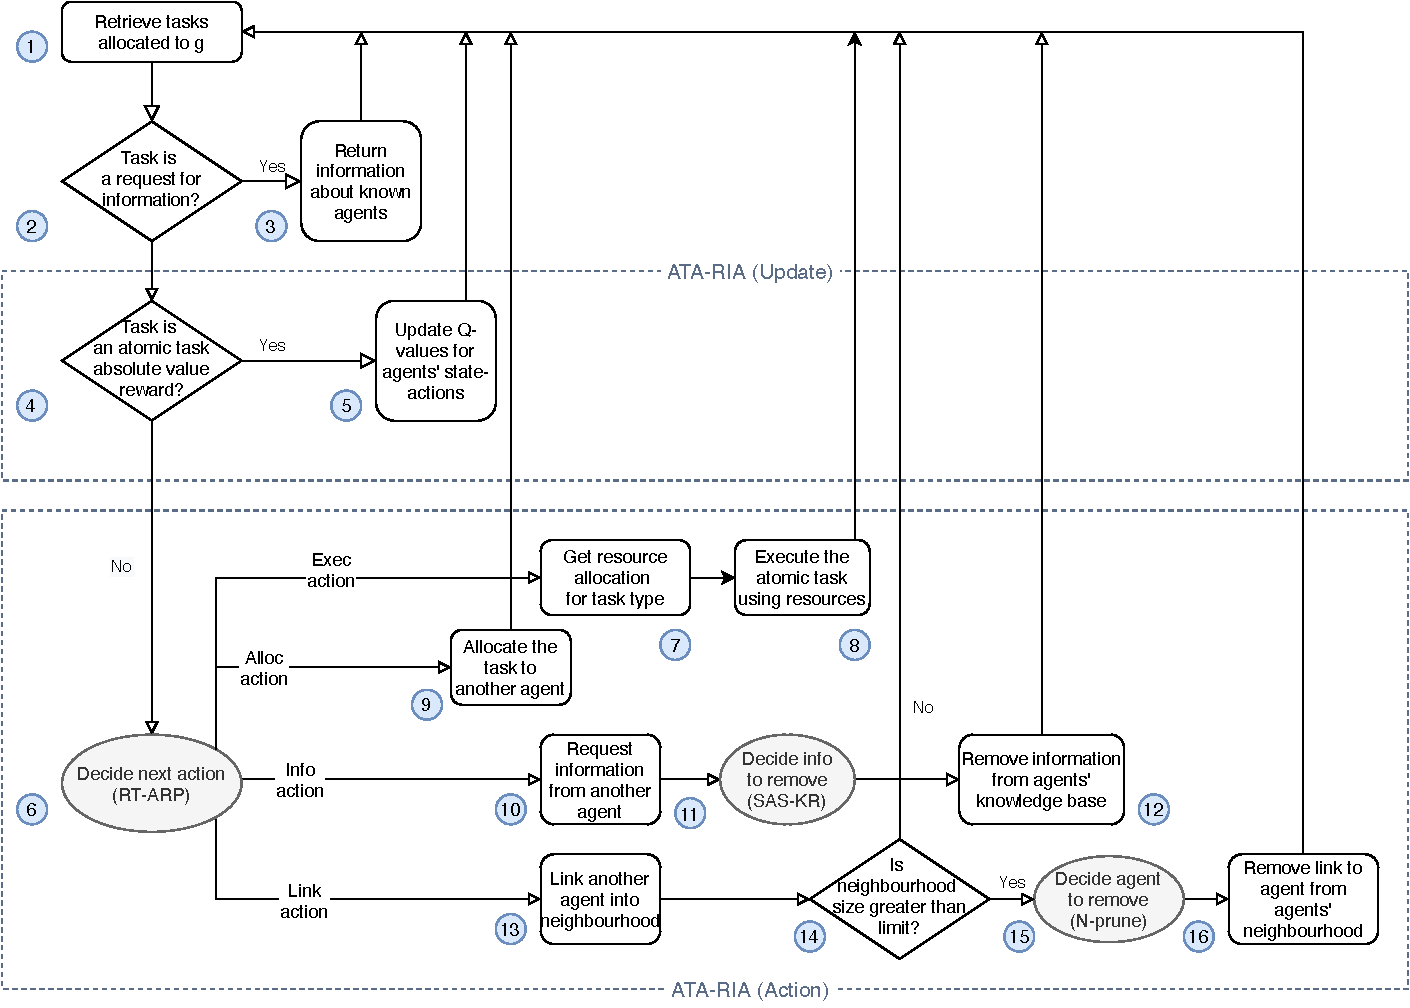
\includegraphics[width=0.8\linewidth, trim={65pt 0pt 65pt 0pt, clip}]{ataria-simplified}
	\caption{\textbf{Simplified \acronymATARIA{}{} flowchart}. The diagram shows the decision-making and actions taken by an agent using the \acronymATARIA{}{} algorithm, including its \acronymRewardTrendsAlgorithm{}{}, \acronymNeighbourhoodPruningAlgorithm{}{}, and \acronymMemoryRetention{}{} sub-algorithms.
}
	\label{fig:ataria-simplified}
\end{figure}

